In this section, we study quantum-to-classical randomness extractors (QC-extractors). The main objective of this section is to answer the following question: how can we extract classical randomness from a physical (quantum) source $\rho_{AE}$ by performing measurements on the quantum state $\rho_A$? Here, $A$ is the accessible quantum source, and $E$ is the environment or eavesdropper correlated with $A$. Similar to the study of classical extractors in \autoref{sec:c_ext}, we want to extract randomness from a quantum source given  min-entropy $H_{\min}(A|E)_\rho \geq k$. It is worth noting that, unlike the classical world, quantum mechanics does allow for the generation of true randomness in case we can prepare the desired quantum source. For example, if we could prepare the state $\ket{+} = {1/\sqrt{2}}(\ket{0} + \ket{1})$ or $\ket{-} = {1/\sqrt{2}}(\ket{0} - \ket{1})$ and measure it in the computational basis\footnote{$\set{\ket{0}, \ket{1}}$ is known as the computational basis of a qubit system, whereas $\set{\ket{+}, \ket{-}}$ is known as Hadamard basis of a qubit system}, i.e., $M_0 = \ket{0}\bra{0}$ and $M_1 = \ket{1}\bra{1}$. Then, we get a \textit{true} random coin. However, this would require preparing the exact source of this form. In general, we want to construct a QC extractor that works for any unknown quantum source as long as it has a sufficiently high min-entropy.

To understand the definition of quantum extractors, consider a classical extractor as a family of permutations acting on the possible values of the source such that it applies a typical permutation from the family to the input for any probability distribution on input bits strings with high min-entropy, which induces an almost uniform probability distribution on a prefix of the output. We define a QQ-extractor similarly in the way that lets the operations be general unitary transformations and the input of the extractor be quantum.

\begin{definition}\textbf{(QQ-extractor \cite{Berta_2014})} 
    Let $A = A_1A_2$ (entangled system) with $n = \log |A|$, define the trace-out map $\Tr_{A_2} : \mathcal{L}(A) \to \mathcal{L}(A_1)$ by $\Tr_{A_2}(\cdot) = \sum_{a_2} \langle a_{2}|(\cdot)|a_{2} \rangle$, where $\{|a_2 \rangle \}$ is an orthonormal basis of $A_2$. For $k \in [-n, n]$ and $\epsilon \in [0,1]$, a $(k, \epsilon)$-QQ-extractor is a set $\{U_1, \dots, U_L\}$ of unitary transformations on $A$ such that for all states $\rho_{AE} \in \mathcal{S}(AE)$ satisfying $H_{min}(A|E)_{\rho} \geq k$, we have 
    
    \begin{align*}
        \frac{1}{L} 
        \sum_{i = 1}^{L} 
        \left\|\Tr_{A_2}(U_{i} \rho_{AE} U_{i}^{\dagger}) - \frac{\I_{A_{1}}}{|A_{1}|} \otimes \rho_{E}\right\|_{1} \leq \epsilon. 
    \end{align*}
    
    where $\log L$ is called the seed size of the QQ-extractor.
\end{definition}

More often than not, we only need a quantum extractor as it is usually sufficient to extract random classical bits. Doing so is much easier than obtaining random qubits. This motivates our need for quantum-classical extractors, where the output system $M$ is measured in the computational basis. Generally, our QC-extractor can be represented as given in \autoref{fig:qc_extractor}. We take a quantum input system with our seed and mix it. Mixing is done with the unitary operation, where we take one basis of the Hilbert space of the quantum system and rotate it into another Hilbert space. After mixing, we use the process of measuring and discarding to generate our classical output system. For that, first, we define the measurement map for $\calH_M \subseteq \calH_N$ as $\calT_{N \to M}: \calH_N \rightarrow \calH_M$,
\begin{align*}
    \calT_{N \to M}(\cdot) = \sum_{m, m'} \bra{mm'} (\cdot) \ket{mm'} \ket{m} \bra{ m }_{M}
    \label{eq:measurement_map}
\end{align*} 
where $\set{ \ket{mm'}}, \set{\ket{m}}$ are orthonormal bases of $\calH_{N}, \calH_{M}$, respectively. We can also observe this map as tracing out $N / M$, and measuring the remaining system $M$ in the basis $\set{\ket{m}}$. Using the above map, we will define quantum-classical min-entropy extractors against quantum side information.

\begin{definition}\textbf{(QC-extractor \cite{Berta_2014})}\label{def:measurement_map}
    Let $A = A_{1} \otimes A_{2}$ (separable system) with $n = \log |A|$. Define the \emph{measurement map} $\calT_{A \to A_{1}}: \calL(A) \to \calL(A_{2})$ by 
    \begin{align}
        \calT_{A \to A_{1}}(\cdot) 
        &= \sum_{a_{1} a_{2}} \bra{a_{1} a_{2}} (\cdot) \ket{a_{1} a_{2}} \ket{a_{1}} \bra{a_{1}},
    \end{align}
    where $\{\ket{a_{1}}\}, \{\ket{a_{2}}\}$ are standard orthonormal bases for $A_{1}, A_{2}$ respectively. 
    
    For $k \in [-n, n]$ and $\varepsilon \in [0, 1]$, a \emph{$(k, \varepsilon)$-QC-extractor} is a set $\{U_{1}, \dots, U_{L}\}$ of unitary transformations on $A$ such that for all states $\rho_{AE} \in \calS(AE)$ satisfying $\Hmin(A|E)_{\rho} \ge k$, we have 
    \begin{align*}
        \frac{1}{L} 
        \sum_{i = 1}^{L} 
        \left\|\calT_{A \to A_{1}}(U_{i} \rho_{AE} U_{i}^{\dagger}) - \frac{\I_{A_{1}}}{|A_{1}|} \otimes \rho_{E}\right\|_{1} \le \eps. 
    \end{align*}
    $\log L$ is called the \emph{seed size} of the QC-extractor. 
\end{definition}

The reason we use this definition is that we want the output of the extractor to be determined by the source and the choice of the seed. In the quantum setting, a natural way of translating this requirement is by imposing that an adversary holding a system that is maximally entangled with the source can perfectly predict the output.

\begin{figure}
    \centering
    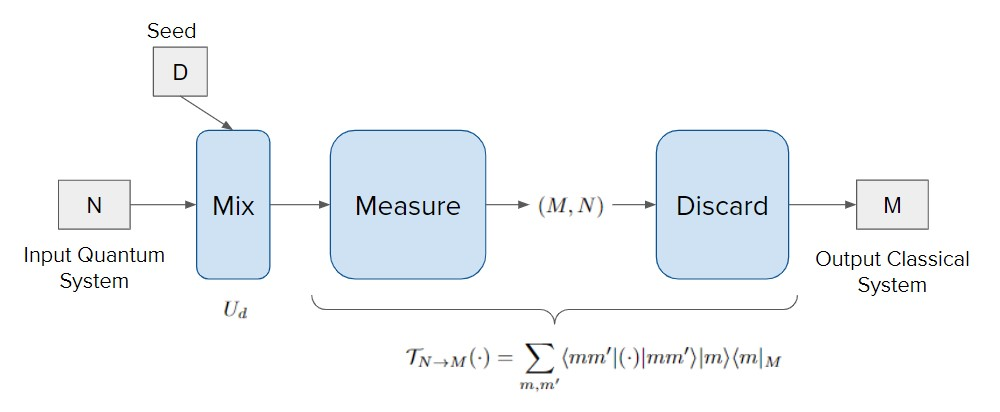
\includegraphics[scale=0.6]{Images/QC_extractor_definition.jpg}
    \caption{Quantum-to-Classical Extractor}
    \label{fig:qc_extractor}
\end{figure}

\subsection{Examples of QC-extractors}
 Two-independent hashing, also known as universal hashing, is one of the most important extractor constructions. We discussed this briefly in \autoref{sec:c_ext}. Basically, it includes selecting two hash functions from a family of hash functions such that it guarantees that the hash codes of both the designated keys are independent random variables \cite{impagliazzo1989pseudo}. In this article, we focus on the theory of unitary $2$-design, which can be seen as the quantum generalization of two-independent hash functions. 


There are many known efficient constructors of unitary $2$-designs [\cite{grossunitary}, \cite{dankert2design}], and in an $n$-qubit space, such unitaries can be computed with circuits of size $O(n^2)$. The following is immediate using a general decoupling result from \cite{dupuisdecoupling,oneshotdecoupling}.

\begin{corollary}
    Let $A = A_{1} \otimes A_{2}$ with $n = \log |A|$. For all $k \in [-n, n]$ and all $\eps > 0$, a unitary $2$-design $\set{U_1, ...., U_L}$ on $A$ is a $(k, \eps)$-QC-extractor with output size 
    $$\log |A_1| = \min{(n, n+k-2\log (1/\eps))}.$$
\end{corollary}
Similar results as above also hold true for "almost" $2$-design unitaries [\cite{osxehrtomamichel}, \cite{oszehrthesis}]. Now, by choosing a reasonably small $L$, making a set of random unitaries, with the seed size of the same order as the output size of the extractor, defines a QC-extractor with high probability. 




\begin{theorem}
    Let $A = A_{1} \otimes A_{2}$ with $n = \log |A|$ and let $\calT_{A \to A_{1}}: \calL(A) \to \calL(A_{2})$ the measurement map defined in \eqref{eq:measurement_map}. Let $\eps > 0$ and $c$ be a sufficiently large constant, and suppose that 
    \begin{align*}
        \log |A_{1}| 
        &\le n + k - 4 \log (1 / \eps) - c \quad \text{and} \quad 
        \log L 
        \geq \log |A_{1}| + \log n + 4 \log (1 / \eps) + c. 
    \end{align*}
    Then, choosing $\{U_{1}, \dots, U_{L}\}$ independently according to the Haar measure \cite{davis1955note} defines a $(k,\varepsilon)$-QC-extractor with high probability.
\end{theorem}

\subsection{Bitwise QC-extractor}
In this section, we discuss constructing simpler unitaries to define a QC-extractor. The construction is composed of unitaries $V$ acting on single qubits followed by permutations $P$ of the computational basis elements. Because the measurement $\calT$ and the permutations $P$ are commutative in nature, we first apply $V$, measure in the computational basis, and then finally apply the permutation  to the classical outcome of the measurement. Unitaries acting on single qubits is frequently a desired attribute for the design of cryptographic protocols, in addition to computational efficiency.

We consider a value $d \geq 2$ as a prime power so that there exists a complete set of mutually unbiased bases in dimension $d$. This set of bases can be represented by a set of unitary transformations given as $\set{V_0, V_1,..., V_d}$ which maps the mutually unbiased bases to some standard basis. The following example, we represent the unitary transformations when we take a full set of mutually unbiased bases in dimension $2$:
\begin{equation*}
    V_0 = 
    \begin{pmatrix}
    1 & 0 \\
    0 & 1 \\
    \end{pmatrix}
    \hspace{1cm}
    V_1 = \frac{1}{\sqrt{2}}
    \begin{pmatrix}
    1 & 1 \\
    1 & -1 \\
    \end{pmatrix}
    \hspace{1cm}
    V_2 = \frac{1}{\sqrt{2}} 
    \begin{pmatrix}
    1 & i \\
    i & -1 \\
    \end{pmatrix}
\end{equation*}

We now define the set $\calV_{d,n}$ of unitary transformations on n qubits as follows:
$$\calV_{d, n} := \set{V = V_{u_1} \otimes ... \otimes V_{u_n} | u_i \in \set{0, 1,..., d}}$$

\begin{theorem}
\label{theorem:bitwiseqc}
    Let $A = A_{1} \otimes A_{2}$ with $|A| = d^{n}$, $|A_{1}| = d^{\xi n}$, $|A_{2}| = d^{(1 - \xi) n}$ and $d$ a prime power. Then, for $\delta \ge 0$ and $\delta' > 0$,
    \begin{multline}
        \frac{1}{|\calP|} \frac{1}{(d + 1)^{n}} 
        \sum_{P \in \calP} \sum_{V \in \calV_{d, n}} 
        \left\|\calT_{A \to A_{1}} \left(P V \rho_{A E} (P V)^{\dagger}\right) - \frac{\I}{|A_{1}|} \otimes \rho_{E}\right\|_{1} \notag \\
        \le \sqrt{2^{(1 - \log(d + 1) + \xi \log d) n} (1 + 2^{- \Hmin^{\delta}(A | E)_{\rho} + z})} 
        + 2 (\delta + \delta'), 
    \end{multline}
    where $\calV_{d, n}$ is defined as above, $\calP$ is a family of pair-wise independent permutation matrices, and 
    \begin{align*}
        z = \log\left(\frac{2}{\delta'^{2}} + \frac{1}{1 - \delta}\right). 
    \end{align*}
    In particular, the set $\{P V: P \in \calP, V \in \calV_{d, n}\}$ is a $(k, \eps)$-QC-extractor provided
    \begin{align*}
        \log |A_{1}| 
        \le (\log(d + 1) - 1) n + \min\{0, k\} 
        - 4 \log(1 / \eps) - 7
    \end{align*}
    and the number of unitaries is $L = (d + 1)^{n} d^{n} (d^{n} - 1)$. 
\end{theorem}

\subsection{Full set of mutually unbiased bases (MUB)}

We saw that QC-extractors are defined by unitary 2-designs. It is reasonable to anticipate that we can create smaller and simpler sets of unitaries if we are simply interested in extracting random classical bits because unitary 2-designs also define QQ-extractors. Here, we build more basic sets of unitaries that define a QC-extractor, using a family of pair-wise independent permutations and a complete set of mutually unbiased bases.

\begin{definition}\normalfont{\textbf{(MUB)}} A \emph{mutually unbiased basis} is defined as the set of unitaries $\set{U_{1}, \dots, U_{L}}$ acting on $A$ such that a state described by a vector $U_{i}^{\dagger} \ket{a}$ of the basis $i$ gives a uniformly distributed outcome when measured in basis $j$ for $i \neq j$. There can be at most $|A| + 1$ mutually unbiased bases for $A$.  
\end{definition} 
\begin{definition}
    A family $\calP$ of of permutations of a set $X$ is called \emph{pair-wise independent} if for all $x_{1} \neq x_{2}$ and $y_{1} \neq y_{2}$, we have \[\Pr[\pi(x_{1}) = y_{1} \hbox{ and } \pi(x_{2}) = y_{2}] = \frac{1}{|X| (|X| - 1)},\]
for any $\pi$ uniformly distributed over $\calP$. 
\end{definition}

Observe that if $X$ is a field (so that $|X|$ is a prime power), the family 
\begin{align*}
    \calP = \{x \mapsto ax + b: x \in X^{*}, b \in X\}
\end{align*}
is pair-wise independent. Observing permutations of the basis elements of a Hilbert space $A$ as a unitary transformation on $A$, we have the following result.

\begin{theorem}
    Let $A = A_{1} \otimes A_{2}$ with $n = \log |A|$, where $|A|$ is a prime power. If $\{U_{1}, \dots, U_{|A| + 1}\}$ defines a full set of mutually unbiased bases, then for $\delta \ge 0$ we have
    \begin{multline}
        \frac{1}{|\calP|} \frac{1}{|A| + 1} 
        \sum_{P \in \calP} \!\!\sum_{i = 1}^{|A| + 1} 
        \left\|\calT_{A \to A_{1}} \left(P U_{i} \rho_{A E} (P U_{i})^{\dagger}\right) - \frac{\I_{A_{1}}}{|A_{1}|} \otimes \rho_{E}\right\|_{1} \notag
       \!\!\leq \sqrt{\frac{|A_1|2^{-H_{\min}(A|E)_{\rho}}}{|A_1|+1} } + 2\delta, 
    \end{multline}
    where $\calP$ is a set of pair-wise independent permutation matrices. In particular, the set $\set{P U_i: P \in \calP, i\in [|A|+1]}$ defines a $(k,\varepsilon)$-QC-extractor provided 
    \[\log|A_1| \leq n+k-2\log(1/\varepsilon),\]
    and the number of unitaries is 
    \[L = (|A|+1)\calP = (|A|+1)|A|(|A|-1).\]
\end{theorem}

The proofs of the above theorems require an understanding of concepts such as one-shot decoupling, permutation extractors, and advanced mathematical tools from linear algebra. Thus, due to page limit restrictions, for proof of the above theorems related to the construction of QC-extractors, we refer the reader to \cite{Berta_2014,berta2013quantum}.

We summarize all the results about QC-extractors in \autoref{table:summary} in the discussion section, i.e., \autoref{sec:discussion}.